% !TeX program = xelatex
\documentclass{aifrontiers}
\usepackage{aifrontiers}
\usepackage[T1]{fontenc}
\usepackage{booktabs}
\usepackage{amsfonts}
\usepackage{nicefrac}
\usepackage{array}
\usepackage{tabularx}
\usepackage{colortbl}
\usepackage{caption}
\usepackage{subcaption}
\usepackage{multirow}
\usepackage{multicol}
\usepackage{float}
\usepackage{wrapfig}
\usepackage{needspace}
\usepackage{placeins}
\usepackage{enumitem}
\usepackage{xspace}
\usepackage{soul}
\usepackage{listings}
\usepackage{algorithm}
\usepackage{algorithmic}

\captionsetup{font=small,skip=6pt}
\captionsetup[table]{position=bottom,font={small,it}}
\captionsetup[figure]{position=bottom,font={small,it}}
\captionsetup[algorithm]{position=bottom,font={small,it}}

% Keep captions and adjacent text comfortably separated without large float gaps.
\setlength{\textfloatsep}{12pt plus 2pt minus 2pt}
\setlength{\floatsep}{10pt plus 2pt minus 2pt}
\setlength{\intextsep}{8pt plus 2pt minus 2pt}
\setlength{\columnsep}{12pt}
\setlength{\emergencystretch}{1em}
\clubpenalty=10000
\widowpenalty=10000
\displaywidowpenalty=10000
\makeatletter
\setlength{\@fptop}{0pt}
\setlength{\@fpsep}{12pt}
\setlength{\@fpbot}{0pt plus 1fil}
\makeatother
\AtBeginEnvironment{thebibliography}{\raggedright}

\lstset{
  basicstyle=\small\ttfamily,
  columns=flexible,
  breaklines=true,
  lineskip=0pt
}

% Cross-reference helpers
\newcommand{\tabref}[1]{Table~\ref{#1}}
\newcommand{\figref}[1]{Figure~\ref{#1}}
\newcommand{\secref}[1]{Section~\ref{#1}}

% Table helpers
\newlength\savewidth
\newcommand\shline{\noalign{\global\savewidth\arrayrulewidth
  \global\arrayrulewidth 1pt}\hline\noalign{\global\arrayrulewidth\savewidth}}
\newcommand{\tablestyle}[2]{\setlength{\tabcolsep}{#1}\renewcommand{\arraystretch}{#2}\centering\footnotesize}

\newcolumntype{x}[1]{>{\centering\arraybackslash}p{#1pt}}
\newcolumntype{y}[1]{>{\raggedright\arraybackslash}p{#1pt}}

\definecolor{baselinecolor}{gray}{0.93}
\newcommand{\baseline}[1]{\cellcolor{baselinecolor}{#1}}

% Keep drafting notes and figure placeholders in source without rendering them.
\newcommand{\addcite}[1]{}
\newcommand{\todo}[1]{}
\newcommand{\figplace}[3]{}
\newcommand{\figwide}[3]{}

% Visible placeholders for sections that have not been drafted.
\newcommand{\sectiontodo}[1]{\textcolor{red}{\textbf{TODO:} #1}}

\renewcommand{\UrlBreaks}{\do\/\do\-}

% Benchmark name and clearly marked draft placeholders.
\newcommand{\benchmark}{PersonaScienceBench\xspace}

\title{PersonaScienceBench: Evaluating Scientific Agents \\ with Diverse Simulated Researchers}
\shorttitle{PersonaScienceBench}
\author{
    {\bfseries Author names to be added} \\[0.45em]
    {\normalsize Affiliations to be added}
}
\date{\today}
\renewcommand{\thefootnote}{\fnsymbol{footnote}}
\renewcommand{\weblink}{}
\renewcommand{\foundrylink}{}
\renewcommand{\hflink}{}
\renewcommand{\ghlink}{}

\begin{document}

\begin{abstract}
Scientific-agent benchmarks increasingly test executable research work, but
usually provide complete specifications or pair agents with one fixed,
cooperative user. In practice, researchers hold undocumented context that an
agent must obtain through conversation. We introduce \benchmark, which holds
the scientific task fixed while varying a simulated researcher. We convert 200
tasks from DiscoveryBench, BixBench, EXP-Bench, SciConvBench, and ASI-Bench
into collaboration tasks that retain each source's deliverable, grader, and
private references. The researcher simulator receives a complete persona
profile that is hidden from the actor; a paired persona-off condition uses the
same protocol without the identity block. Independent repeated episodes
separate collaborator effects from ordinary run variation. Native benchmark
scores measure scientific correctness, while interaction metrics measure
review, clarification, revision, communication, and language adaptation.
Because the persona panel was selected using exploratory pilot outcomes, it
characterizes a range of collaborator effects rather than a population
average. \benchmark provides a controlled test of whether scientific-agent
performance depends on whom the agent collaborates with.

\end{abstract}
\maketitle

\section{Introduction}
\label{sec:introduction}

\paragraph{Scientific work is collaborative.}
Language-model agents now perform substantial parts of the scientific
workflow. They search literature, propose hypotheses, write and execute
analysis code, and assemble results into reports
\citep{lu2024aiscientist,yamada2025aiscientistv2,gottweis2025coscientist,mitchener2025kosmos}.
The benchmarks used to measure this progress have followed the same
trajectory, moving from recall and reasoning questions toward executable
analysis tasks drawn from real studies
\citep{majumder2024discoverybench,mitchener2025bixbench,kon2025expbench,ye2025replicationbench}.
Yet in practice these systems function as co-scientists rather than
autonomous investigators, and the case has been made that they are not
architecturally built for unsupervised discovery \citep{bisht2026notbuilt}.
A deployed scientific agent sits inside a collaboration: someone designed
the experiment, ran the instrument, and holds the context that determines
whether an analysis is valid. That context is frequently undocumented. Which
plates were processed on a different day, why three samples were dropped,
whether a covariate is confounded with batch, which normalization the lab
actually applies---these facts live with the researcher, not in the data
directory. The agent's scientific output therefore depends not only on its
own reasoning but on an exchange with a particular human who may explain
readily, answer only what was literally asked, or misremember a detail.

\paragraph{The evaluation gap.}
Most scientific agent benchmarks specify each task completely and
uniformly, which measures capability under ideal information but says
nothing about capability under realistic information transfer. A recent line
of interactive benchmarks closes part of this gap by requiring agents to
recognize underspecification and ask: HiL-Bench measures whether coding
agents escalate at the right moments \citep{trinh2026hilbench},
SciConvBench evaluates multi-turn clarification for ill-posed computational
science requests \citep{somasekharan2026sciconvbench}, and work in
tool-agent settings evaluates interaction with a simulated user under
domain rules \citep{yao2024taubench,chen2026appworldul,ta2026regretbench}.
These benchmarks establish that asking is hard. They do not, however, vary
\emph{whom} the agent is asking. The simulated collaborator is typically a
single cooperative interlocutor with one disclosure policy, so the
collaborator is a fixed property of the environment rather than an
experimental condition. The closest departures from this pattern vary
designed behavioral axes---non-collaborative user simulators degrade tool
agents through impatience, digression, and incomplete utterances
\citep{shim2025noncollaborative}, and evolved persona policies induce
realistic behavioral variation in otherwise cooperative simulators
\citep{chopra2026ppol}---but do so in retail, airline, and customer
service domains where there is no scientific ground truth to get wrong.
The result is that three distinct sources of difficulty remain entangled in
current evaluation: the intrinsic difficulty of the scientific task, the
capability of the agent, and the character of the collaborator the agent
happens to be working with. Reporting a single score against a single
default collaborator silently averages over the third.

\paragraph{Our approach.}
This paper introduces \benchmark, a benchmark that holds the scientific
task fixed and varies the simulated researcher. We convert 200 tasks from
five scientific agent benchmarks---DiscoveryBench, BixBench, EXP-Bench,
SciConvBench, and ASI-Bench---into collaboration tasks, preserving each
source's native deliverable and grading rules rather than reducing them to
a common format. An actor agent must produce that native deliverable while
interacting with a simulated researcher through a shared review protocol.
The researcher is conditioned on a complete rendered profile drawn from
MatrAIx, a population-scale simulated-user infrastructure whose persona
records span 1,290 categorical dimensions covering background, psychology,
capability, and behavior \citep{li2026matraix}. Our renderer emits the
populated attributes as an explicit attribute--value listing grouped by
category, so a condition is a fully auditable set of stated attributes rather
than authored prose; a single profile typically contributes on the order of two
hundred such attributes. The profile is injected verbatim into the researcher
simulator's system prompt only, without truncation or projection onto the
task domain, so the actor observes personality solely through conversation.
Every task is also run with the identical protocol and the
identity block removed, giving a paired persona-off control that separates
collaborator variation from task difficulty. Evaluator references stay
private throughout, and each task--condition cell is repeated across
independent episodes so that persona effects can be distinguished from
ordinary run-to-run variation. Because the same task is scored under
multiple collaborators with a shared baseline, differences are attributable
to the collaborator rather than to task selection.

Upstream validation of this persona corpus establishes that conditioning
reliably induces declared behavior---91.5\% of trials in a controlled
adherence study---but does so in Survey, Chatbot, Web, and App environments
over a task library concentrated in commerce, software, finance, and
healthcare \citep{li2026matraix}. Scientific research collaboration is not
among those environments, and product feedback rather than scientific
correctness is the measured outcome. \benchmark supplies that missing
environment and asks the question it enables: whether persona-induced
behavioral variation propagates into graded scientific error.

\paragraph{What we measure.}
Evaluation is deliberately two-sided. Outcome metrics use each source
benchmark's native grader, so a persona effect registers as a change in
scientific correctness and not merely as a change in conversational tone.
Interaction metrics---review rounds, revisions, questions asked,
clarification coverage, message length, and language adaptation---are
recorded separately, because a collaborator can change an agent's behavior
substantially without changing its score, and can change its score without
changing observable behavior. Keeping these separate is what allows a
failure under a difficult collaborator to be diagnosed as a failure to
obtain available information rather than assumed to be one.
\todo{Insert the principal quantitative findings once the repeated-run
analysis over the full persona panel is complete: direction and magnitude of
persona effects with confidence intervals, which benchmarks and fields are
most sensitive, and whether behavioral divergence tracks outcome divergence.
Pilot runs showed score changes in both directions of substantial magnitude
relative to the shared baseline, but that panel was outcome-selected and is
reported as a selection stage, not as an effect estimate.}

\paragraph{Contributions.}
\begin{itemize}[leftmargin=1.5em]
  \item \textbf{A persona-conditioned scientific collaboration benchmark.}
  We convert 200 tasks from five scientific agent benchmarks into
  interactive collaboration tasks under a source-preserving contract that
  retains native deliverables, graders, and private references
  (\secref{sec:benchmark}).
  \item \textbf{An experimental design that isolates the collaborator.}
  Full-profile researcher conditioning, a paired persona-off control on the
  identical protocol, and repeated independent episodes per cell yield
  paired comparisons in which the researcher is the manipulated variable
  (\secref{sec:experimental-setup}). We document the two-stage profile
  selection, including its outcome-dependent final stage, rather than
  presenting the panel as population-representative.
  \item \textbf{An empirical characterization of collaborator sensitivity.}
  We report outcome and interaction effects with repeat-based uncertainty,
  their dependence on task format and scientific field, and
  evidence-linked conversation cases tracing profile wording to researcher
  behavior, actor decisions, and graded outcomes
  (\secref{sec:results},~\secref{sec:discussion}). Completed experiments
  are reported separately from proposed extensions.
\end{itemize}

\noindent
\secref{sec:related-work} positions this work against scientific agent
benchmarks, interactive and simulated-user evaluation, and persona
simulation. \secref{sec:benchmark} defines the benchmark,
\secref{sec:experimental-setup} the experimental protocol,
\secref{sec:results} the results, and \secref{sec:discussion} mechanism
evidence from conversation traces. \secref{sec:limitations} states what
simulated collaborators and an outcome-selected panel cannot establish.

\section{Related Work}
\label{sec:related-work}

\subsection{Scientific Agent Benchmarks}
Benchmarks for scientific agents have moved from knowledge recall toward
executable research work, and the five sources converted in \benchmark span
the range of task objectives this shift produced. DiscoveryBench frames
data-driven discovery as hypothesis search and verification over provided
datasets, with tasks derived from published findings and graded against
reference hypotheses \citep{majumder2024discoverybench}. BixBench supplies
real bioinformatics analysis capsules and requires agents to execute
multi-step computational biology workflows and answer open-ended questions
about the data \citep{mitchener2025bixbench}. EXP-Bench targets the
experimental process itself, decomposing research experiments extracted
from publications into design and implementation subtasks
\citep{kon2025expbench}. ASI-Bench progressively withdraws methodological
guidance across matched conditions to test autonomous execution
\citep{zhou2026asibench}. SciConvBench, discussed further below, is the
only one of the five whose native format is dialogue rather than artifact
production \citep{somasekharan2026sciconvbench}. Related efforts scale task
collection automatically \citep{li2025autosdt} or test faithful replication
of published analyses \citep{ye2025replicationbench}.

These benchmarks differ substantially in deliverable and grading, which
motivates our source-preserving conversion contract: reducing them to a
common answer format would discard exactly the native scoring that makes a
persona effect interpretable as a scientific error. Their information regimes
also differ: most use one fixed specification, ASI-Bench varies the amount of
methodological guidance, and SciConvBench makes clarification native. None
manipulates collaborator identity and behavior while holding the scientific
task and scoring procedure fixed. \benchmark retains these tasks and their
graders while making that collaborator the experimental variable.

\subsection{Interactive Agents and Simulated Users}
A growing body of work evaluates agents that must interact rather than
execute a complete specification. $\tau$-bench emulates dynamic
conversations between an agent and a language-model user under
domain-specific rules \citep{yao2024taubench}, extended by $\tau^2$-bench to a
dual-control setting in which both agent and user can act on the environment
\citep{barres2025tau2bench}, and AppWorld-UL constructs
tasks that require clarification, confirmation, and infeasibility reporting,
simulating the user with explicitly designed knowledge boundaries
\citep{chen2026appworldul}. In the science and engineering setting,
SciConvBench evaluates multi-turn clarification for ill-posed computational
science requests across fluid mechanics, solid mechanics, materials
science, and PDE formulation, scoring dialogue quality by rubric-based judge and
explicitly requiring no solver, code execution, or tool invocation for scoring
\citep{somasekharan2026sciconvbench}. HiL-Bench isolates the judgment of
\emph{when} to escalate, showing that coding agents which succeed given
complete context degrade sharply when they must themselves decide whether
information is missing \citep{trinh2026hilbench}. Clarification has also
been formalized as a sequential decision problem over whether, what, and
when to ask \citep{ta2026regretbench}, and user simulation has been used to make
agent evaluation more efficient by guiding it toward behavioral diversity
\citep{nakash2026diversity}.

Our work departs from this literature in what is held constant. These
benchmarks fix the human and vary the task, measuring whether the agent
asks well. \benchmark fixes the task and varies the human, measuring how
much of the scientific outcome is attributable to the collaborator. Two
recent lines vary the simulated user deliberately. Non-collaborative user
simulators inject requests for unavailable services, digressions,
impatience, and incomplete utterances, and show state-of-the-art tool
agents degrading substantially under each condition
\citep{shim2025noncollaborative}. Persona Policies argue that LLM-based
simulators inherit the cooperative and homogeneous behavior of their base
models, and search for persona generator programs that induce realistic
behavioral variation while preserving task goals, reporting large fitness
gains and improved agent robustness on $\tau^2$-bench retail and airline
domains \citep{chopra2026ppol}. Together these establish the effect we
investigate: varying the simulated human changes measured agent performance.
Both, however, operate in retail, airline, and customer-service domains,
where a failure is a dialogue breakdown or an incorrect transaction, and both
vary hand-designed or search-discovered behavioral axes rather than
integrated researcher profiles. We instead measure consequences on native
scientific graders, where a collaborator effect surfaces as an incorrect
hypothesis, a flawed analysis, or an unsubmitted deliverable. User simulation for evaluating interactive systems
long predates this literature, from early user models for spoken dialogue
evaluation \citep{eckert1997usermodeling} through agenda-based simulators for
dialogue policy learning \citep{schatzmann2007agenda} to LLM-based behavioral
simulation at scale \citep{wang2023userbehavior}.

\paragraph{Validity of the simulator itself.}
A parallel line of work questions whether LLM user simulators behave as their
specification requires, and it bears directly on our design rather than only on
our citations. Simulators exhibit \emph{assistant bias}, drifting toward helpful
assistant behavior rather than sustaining the user role
\citep{jeong2026assistantbias}---a concern for a researcher simulator whose job
includes gatekeeping and refusal rather than assistance. Bounding what a
simulated user knows is also harder than a prompt instruction suggests, and
naive persona instructions do not reliably constrain a simulator's effective
knowledge \citep{balog2026bounding}. Separately, distributing a task across
multiple turns can reduce model reliability \citep{laban2025lost}, making
interaction length a potential confound for protocols with several review
rounds. We treat these as threats to the manipulation rather than as background,
and \secref{sec:limitations} states how each bounds our claims.

\subsection{Persona-Conditioned Simulation}
Conditioning language models on personal descriptions to elicit distinct
behavior has an established basis. Argyle et al.\ showed that conditioning
on socio-demographic backstories reproduces response distributions of human
subgroups, terming this algorithmic fidelity \citep{argyle2022outofone}. At
scale, Persona Hub demonstrated that a large collection of diverse persona
descriptions can drive correspondingly diverse model outputs
\citep{ge2024personahub}, and subsequent work studies how much generated
diversity persona detail actually produces
\citep{kambhatla2025lexicaldiversity}. For evaluation specifically, Persona
Generators optimize for coverage of the space of possible users rather than
density matching of the most probable ones
\citep{paglieri2026personagenerators}, and frameworks have been proposed to
measure whether persona simulation is faithful along adherence, consistency,
and naturalness \citep{bao2026eval4sim}.

\paragraph{Relation to MatrAIx.}
The researcher profiles used in \benchmark are drawn from MatrAIx, a
population-scale simulated-user evaluation infrastructure
\citep{li2026matraix}. Its Persona 8B corpus represents human variation
through a shared schema of 1,290 categorical dimensions spanning background,
psychology, capability, behavior, and lifestyle. Records are either sampled
from a dependency graph that preserves correlated attributes and enforces
compatibility rules, or extracted from human-authored sources---Wikipedia
biographies, Amazon review histories, the Stack Overflow Developer Survey,
the General Social Survey, PRISM Alignment profiles, and consented survey
responses---mapped into the same schema and de-identified. The upstream release
also attaches natural-language descriptions to human-grounded records, but our
renderer does not use them: the injected identity block is an explicit
attribute--value listing grouped by category, typically on the order of two
hundred populated attributes for a single profile. A condition is therefore a
fully auditable set of stated attributes rather than authored prose, which is
what allows observable behavior to be checked against exact profile text. A
quality-filtered public coreset of
approximately one million records is released, comprising 599,847
human-grounded and 400,000 synthetic personas.

MatrAIx also supplies the strongest existing evidence that this form of
conditioning works: in a 400-trial controlled adherence study spanning ten
behavioral attributes, declared behavior was expressed or correctly
suppressed in 91.5\% of trials \citep{li2026matraix}. That study, however,
was conducted in the four environments MatrAIx provides---Survey, AI
Chatbot, Web, and App---across a task library concentrated in Commerce,
Software, Finance, and Healthcare. Scientific research collaboration is not
among them, and product feedback rather than scientific correctness is the
measured outcome; related demonstrations of persona-based simulation target
the same interactive-application settings \citep{liu2026personaeval}.
\benchmark extends this line of work in exactly that direction. We take the
persona population as given and validated at the level of behavioral
adherence, then ask a question the upstream infrastructure does not: whether
persona-induced behavioral variation propagates into \emph{graded scientific
error} when the simulated human is a research collaborator and the task is
scored by a native scientific verifier. Our contribution is therefore the
scientific environment, protocol, and outcome measurement, not the persona
corpus or its construction.

\paragraph{Caveats adopted from this literature.}
A review of 63 persona studies found that task and target population are
frequently underspecified and that only about a third discuss the
representativeness of their personae, proposing a transparency checklist in
response \citep{batzner2025whosepersonae}. Analytic flexibility in
simulating human data is substantial enough that defensible configuration
choices materially change fidelity conclusions
\citep{cummins2025analyticflexibility}. Work in a scientific domain is
directly instructive: when synthetic personas evaluated a genomics
visualization system, grounded personas shifted toward the concerns of
documented users while ungrounded ones drifted toward issues real experts
never raised, and both missed a preference the expert study observed
\citep{nguyen2026sycamore}. The MatrAIx release is itself explicit that its
human-grounded records are not population-representative, that calibration
targets only four marginal distributions rather than joint coverage over all
1,290 dimensions, and that human studies remain necessary before applying
conclusions to real populations \citep{li2026matraix}. We therefore treat our
profiles as controlled stimuli that induce reproducible interaction
conditions, not as substitutes for human researchers, and we do not interpret
demographic attributes of a profile as properties of any real group.
Additionally, because we inject complete profiles rather than manipulating
individual schema dimensions, communication style, availability, and domain
knowledge vary together within a condition; \secref{sec:limitations} treats
this full-profile confounding directly.

A further distinction from this literature clarifies our architecture.
Persona-conditioned simulation separates the relatively persistent
\emph{persona}---background, identity, values, skills, personality, enduring
preferences---from the more changeable \emph{user state} that many behaviors
actually depend on, including a current goal, available knowledge, prior
interactions, trust, and frustration \citep{liu2026fitnessforpurpose}.
Scientific collaboration requires both: a researcher's disposition is
persistent, but what they know about \emph{this particular study} is not a
property of their biography. \benchmark separates these sources accordingly.
The persona supplies persistent disposition and is the manipulated variable;
study-specific context is owned by the task and held identical across
persona conditions; and private evaluator references are withheld from the
researcher entirely. A profile therefore changes how study context is
communicated and reviewed, not what ground truth exists, which is what makes
a score difference interpretable as a consequence of collaboration rather
than of unequal information endowment.

This separation is imperfect in one respect worth stating. The MatrAIx schema
is not purely dispositional: rendered profiles include a small
\emph{interaction state} group with fields such as the participant's expertise
gap relative to the system, work schedule, and work location. At least one such
field is potentially consequential, since a profile that declares its holder an
expert testing the system frames the interaction differently from one seeking
genuine assistance. These fields are part of the injected condition and are not
separately manipulated, so the persona conditions carry a limited amount of
state alongside disposition.

\subsection{Evaluating Collaboration}
Evaluations of interactive agents tend to report either outcome scores or
interaction quality, and the two can diverge. Outcome-only scoring cannot
distinguish an agent that obtained the information it needed from one that
was simply given an easier collaborator; interaction-only scoring, as in
rubric-graded clarification dialogues, establishes that an agent asked
sensible questions without establishing that the resulting science was
correct \citep{somasekharan2026sciconvbench}. Metrics that combine the two,
such as HiL-Bench's pairing of task success with the precision and recall
of escalation decisions, come closer by asking whether the agent asked
about the things that actually mattered \citep{trinh2026hilbench}.

\benchmark reports native outcome scores and interaction metrics as separate
quantities over the same episodes, with a paired persona-off baseline and
repeated independent episodes per cell. This supports three claims that a
single aggregate cannot: that a collaborator changed observable agent
behavior, that a collaborator changed graded scientific correctness, and
that these two need not co-occur. We additionally analyze stage-aligned
conversation trajectories and present evidence-linked cases tracing profile
wording through researcher behavior to actor decisions and graded outcomes.

\paragraph{Which validity we claim.}
A fitness-for-purpose framework for persona-conditioned simulation argues
that simulated users should be judged against the specific claim they were
built to support rather than against general human-likeness, and distinguishes
four forms of validity: persona fidelity, whether the model preserves and
uses the supplied profile; behavioral and interaction validity, whether
actions and trajectories resemble the target human process; task and
ecological validity, whether evaluation with simulated users exposes the same
capabilities and failures real users would reveal; and distributional
validity, whether a collection of simulated users represents an intended
population \citep{liu2026fitnessforpurpose}. Passing one form does not imply
the others, and the framework's central recommendation is to state exactly
what has been validated \citep{li2026humansimulation}. We adopt that
discipline. \benchmark inherits persona fidelity from upstream adherence
validation \citep{li2026matraix} rather than re-establishing it, and its own
contribution is evidence about task validity in a new domain: whether
collaborator variation exposes scientific failures that a single default
collaborator does not. We explicitly do not claim distributional validity.
The final profile panel was selected using pilot outcomes, so it characterizes
the range of collaborator effects rather than estimating an average effect
over any researcher population, and we make no claim that behavioral and
interaction validity holds against real scientist behavior, which would
require human comparison data we do not have. \secref{sec:limitations}
develops these constraints.


\section{PersonaScienceBench}
\label{sec:benchmark}

\subsection{Task and Interaction Formulation}
A \emph{task} is a scientific problem drawn from a source benchmark,
retaining that source's native deliverable and grading contract. An
\emph{actor} is the agent under evaluation; it holds the tools, executes
code where the track requires it, and produces the deliverable. A
\emph{simulated researcher} is a language model that plays the collaborating
scientist: it reviews the actor's proposed approach, answers questions,
requests revisions, and decides when the work may conclude. A \emph{persona
condition} assigns that researcher either a complete rendered profile or, in
the control condition, no identity block. An \emph{episode} is one complete
interaction from the original task statement to a sealed deliverable. An
\emph{evaluator} is the source benchmark's native grader, which runs after
the episode is sealed and never participates in the conversation.

Three information domains are kept separate by construction. \emph{Public
task context} is supplied identically in every condition and is owned by the
task, not the persona; it includes the scientific question, the input files,
and the required output format. \emph{Researcher-held information} is what the
simulated researcher can supply on request, which creates the reason to
interact at all. \emph{Private references} are the evaluator's answer keys and
grading rubrics, which are withheld from both actor and researcher throughout.
Because study-specific context is task-owned and held fixed, a persona changes
how that context is communicated, prioritized, and reviewed, but not what
ground truth exists or what information is in principle obtainable. This is
what licenses reading a score difference as a consequence of collaboration
rather than of unequal information endowment across conditions.

\figwide{1.3in}{benchmark-overview}{Placeholder: benchmark construction, context separation, and the actor--researcher--evaluator workflow.}

\subsection{Scientific Tasks and Source Conversion}
Conversion is governed by a source-preserving contract: each task keeps its
native deliverable, its native grader, and its native notion of success.
Tasks are not rewritten into a common answer format, because doing so would
discard the source-specific scoring that makes a persona effect legible as a
scientific error rather than as a conversational difference.

Four sources use an execution or design track under a shared active-researcher
protocol. DiscoveryBench tasks require the actor to produce a hypothesis
specified as context, variables, and relationship, given datasets, metadata,
and a discovery goal; its real-world split is manually derived from published
papers, while a larger synthetic split is model-generated for controlled
difficulty \citep{majumder2024discoverybench}. We retain its native
hypothesis-match grading, and note that the analysis workflow is an optional
output that the native metric does not score, so a workflow produced during
collaboration is retained as evidence rather than graded. BixBench tasks place
the actor in an empty notebook inside a provisioned environment and require
multi-step exploration of heterogeneous input files to answer expert-authored
questions; the primary regime is open answer, judged binary-correct against a
reference answer rather than by numeric tolerance
\citep{mitchener2025bixbench}.

ASI-Bench requires scientific implementation and execution scored by per-task
programmatic gates and weighted scorers against a reference solution, and it
natively varies \emph{how much methodological guidance the task supplies},
through matched levels ranging from a full method statement down to an
objective alone \citep{zhou2026asibench}. Our conversion exploits that
structure directly, and it is the source in which this benchmark's mechanism is
most literally instantiated: the actor receives the objective-only prompt,
while the withheld methodological guidance from the next-richer level is
assigned to the \emph{researcher} as optional advice the actor can obtain only
by asking. Guidance facts are extracted only from explicitly named
methodological sections and the richest guidance level is never transferred
wholesale, so the researcher holds method-level consultation rather than a
complete solution. The resulting condition is objective-only execution with
methodological consultation available on request, which is by construction not
autonomous objective-only execution, and ASI-Bench numbers reported here are
therefore not comparable to native autonomous results at that level. Because
the frozen panel draws 40 tasks from a benchmark of roughly 60, source coverage
is substantially higher here than for the other four sources.

EXP-Bench natively requires an agent to implement \emph{and execute} a research
experiment reconstructed from a published paper, with ground truth spanning
design, implementation, and conclusion components
\citep{kon2025expbench}. We convert it into a \textbf{design-only} track, and
this is a modification of the benchmark rather than a mode it provides: we
retain only its design ground truth and its design-correctness criterion, and
the actor produces an experimental design and controlled comparison plan
without executing the experiment. Execution-dependent components of the native
ground truth are therefore not scored in our conversion, and EXP-Bench results
reported here are not comparable to native EXP-Bench leaderboard numbers. Our
configuration additionally averages three judge passes per deliverable to
reduce grading variance; these are repetitions of \emph{our} grading
configuration, not part of the native EXP-Bench protocol, and they are not
independent episode trials.

SciConvBench is preserved as a dialogue track rather than being converted into
an artifact task. It retains its native ambiguous or internally inconsistent
request and its intended-specification split: the actor asks clarification
questions or returns a completion signal, with up to ten question turns and a
final attempt, and native judges assess specification recovery, intent
preservation, and conversational grounding. No scientific solver is executed.
Converting SciConvBench into a full-specification copying test would have
removed exactly the interactive difficulty it was built to measure.

\paragraph{Source pinning and leakage control.}
Every source is pinned by revision, and the datasets that ship reference
material alongside inputs require explicit leakage control. Source repositories
and dataset revisions are recorded by commit hash with per-file SHA-256
checksums, because at least one source has been revised after publication in
ways that change measured performance: the BixBench dataset was substantially
re-reviewed after its paper appeared, with questions revised for answerability
and the schema flattened, so scores are comparable only within a pinned
revision and results here are not comparable to the numbers reported in the
original paper \citep{mitchener2025bixbench}. BixBench capsule archives also
bundle the analyst's executed solution notebook alongside the input data, which
would leak answers directly into the actor's workspace. Our conversion mounts
only data members: files whose path components match reference-material
patterns are excluded, gold notebooks remain in the immutable archive outside
both actor and researcher mounts, and the researcher-visible context is
generated from input headers, labels, formats, and identifier examples without
reference to any gold notebook, hypothesis, result, or ideal answer. Where a
native grader does not verify an execution artifact, this is recorded rather
than assumed.

\subsection{Sampling and Scientific Coverage}
The task panel is a frozen random sample of 200 tasks, 40 from each source,
drawn with seed 20260929. The selection manifest is content-addressed by
SHA-256 \texttt{74619131\allowbreak 2aa95b39\allowbreak a1b04117\allowbreak
1b14e0a9\allowbreak 2dd97d7c\allowbreak b68f6d39\allowbreak d719d6bc\allowbreak
6fd20b06\allowbreak 533} and the identical panel is used for every condition and
every trial; tasks are never resampled between trials.

The sampling policy admits numerical scientific workflows and permits
diagnostic plots as intermediate artifacts, while excluding image-centric
objectives such as image interpretation, microscopy analysis, reconstruction,
computer vision, video, and visual generation. Screening was applied to
scientific objectives and required outputs, not only to input file types.
Eligibility screening and successful input preparation do not guarantee
successful execution or grading, and tasks that fail technically remain
visible as outcomes rather than being replaced.

Equal per-source quotas define the design. The resulting distribution over
scientific super-families is an empirical consequence of that design, not a
field quota: 50 life sciences, 63 physical sciences and engineering, 55
mathematics and computer science, and 32 social sciences and humanities. By
answer format the panel contains 80 empirical analyses, 40 designs, 40
specification dialogues, and 40 scientific implementations.

Source and field are therefore partly confounded, and this constrains
interpretation throughout. All selected social-science and humanities tasks
come from DiscoveryBench, and BixBench dominates the life sciences. Field
effects and format effects cannot be fully separated in this panel;
comparisons within a single source and format are reported where coverage
permits. Subfield, source-study, and task-family tags are retained in the
manifest, and multiple tasks may derive from a single source study, so tasks
are not treated as independent studies for uncertainty estimation.

\begin{table}[t]
  \centering
  \caption{Task allocation in the frozen panel. Equal per-source quotas define the design; super-family counts are the empirical distribution of the frozen sample rather than field quotas.}
  \label{tab:task-coverage}
  \begin{tabularx}{\columnwidth}{@{}lr>{\raggedright\arraybackslash}X@{}}
    \toprule
    Benchmark & Tasks & Native deliverable \\
    \midrule
    DiscoveryBench & 40 & Hypothesis (context, variables, relationship) \\
    BixBench & 40 & Open answer from notebook analysis \\
    EXP-Bench & 40 & Experimental design (design-only conversion) \\
    SciConvBench & 40 & Specification recovery dialogue \\
    ASI-Bench & 40 & Execution with researcher-held guidance \\
    \midrule
    Total & 200 & \\
    \bottomrule
  \end{tabularx}
\end{table}

\subsection{Researcher Profiles and Selection}
Profiles are complete rendered MatrAIx persona records
\citep{li2026matraix}, injected verbatim into the researcher simulator's
system identity. No truncation, summarization, or projection onto the task
domain is applied, and the same profile text is used for every task and every
trial. Neither the actor nor the evaluator receives the profile.

Selection proceeded in two stages, and the second is outcome-dependent. In the
first stage, an original sample of 300 profiles was rescreened to 180 eligible
records, from which a source-balanced, behaviorally diverse cohort of 30 was
selected \emph{without} reference to model scores. An exploratory pilot then
ran all 30 profiles plus the persona-off control. In the second stage, ten
profiles were selected by \emph{largest absolute deviation} from the
persona-off baseline in that pilot---not by highest score---giving, in ranked
order, 046, 003, 004, 089, 001, 127, 262, 224, 148, and 026. This panel
deliberately contains deviations in both directions. Persona 155 is retained as
an additional comparison condition outside the top-ten set and is labeled
separately in all analyses.

This selection is disclosed rather than presented as representative. Because
the panel was chosen using pilot outcomes, it characterizes the \emph{range} of
collaborator effects and must not be read as an unbiased estimate of an average
effect over any researcher population; the pilot scores that drove selection are
not evidence that these profiles are optimal on new tasks. Profiles are not
reselected using results from the expanded campaign.

\todo{Add the compact persona table: for each of the ten selected profiles plus
155, give domain background, methodological familiarity, communication language,
and observable workflow preferences, with links to the exact injected prompt
text and profile hashes. Two illustrative entries are available now---148 is a
senior medical researcher with medicine and statistics background, English
communication, extensive detail, accuracy-first working style, and demanding
approval behavior; 155 has an agriculture/agronomy and management background,
Mandarin communication, concrete detailed guidance, structured teamwork, and a
preference for familiar methods---but the remaining nine must be described from
their exact injected text rather than paraphrased from selection metadata.}

Two cautions apply to reading these profiles. Full profiles contain many
attributes and are sometimes internally inconsistent, so observable behavior
must be evaluated against the actual injected text rather than against a
demographic label or an assumed expertise level. And because complete profiles
are injected, communication style, availability, and domain knowledge covary
within a condition; this study does not isolate individual traits or
demographic effects (\secref{sec:limitations}).

\subsection{Collaboration Protocol and Isolation}
The four execution and design tracks share an active-researcher protocol in
which approach review and result review are mandatory. An episode proceeds in
five stages: the researcher requests input inspection and a proposed approach;
the actor reports a plan with evidence, assumptions, and uncertainties; the
researcher approves the approach or requests a focused clarification; the actor
performs the analysis or writes the design and submits a result handoff; and
the researcher requests an identifiable revision or concludes, after which the
controller seals the deliverable for separate native grading. Each episode
allows twelve researcher requests and sixty actor calls. Missing submissions
remain explicit outcomes and are not silently excluded.

Because plan and result handoffs are mandatory in this interface, handoffs must
not be counted as spontaneous engagement. Extra review requests measure
\emph{simulator} activity; questions or new proposals raised inside actor
handoffs measure \emph{actor} initiative. These are reported as separate
quantities. Shared handoffs contain actor-selected evidence only: the
researcher does not automatically inspect private tool logs, so what the
researcher knows about the analysis depends on what the actor chose to
surface.

One protocol asymmetry is recorded because it affects interpretation. The
controller permits termination only during result review, so an unreadable or
malformed input can trap a cautious researcher in approach review. This
behavior is preserved rather than patched mid-campaign, since altering it would
require a new run version and break comparability with completed episodes.

SciConvBench retains its native workflow, with the persona conditioning the
simulated user's answers. One consequence is analytically important: the
actor's \emph{first} question necessarily precedes any persona-conditioned
reply, so changes in actor activity attributable to the persona must be
measured only after the first researcher response.

Isolation is enforced on three boundaries. The persona reaches only the
researcher simulator. Private evaluator references, hidden graders, and
credentials remain outside both actor and simulator access. General knowledge
is available to the simulator in all conditions, including persona-off, so the
control differs from the persona conditions only by the presence of the
identity block. Episodes execute in isolated environments, and full shared
messages, model requests and responses, tool events, submissions, native
grades, and termination reasons are recorded for every episode, including
failed ones. Legacy optional-question bridge interfaces remain implemented for
compatibility but constitute a different interaction condition and are not used
here.

\section{Experimental Setup}
\label{sec:experimental-setup}

\sectiontodo{Describe the experimental setup.}

\section{Results}
\label{sec:results}

\subsection{Model-Level Scientific Collaboration}
\label{sec:model-results}
% Model rows and provider layout: Overleaf commit 3aa9990.
% Haiku: preserve local results updated 2026-10-06 (behavioral means and CIs supplied by collaborator, 2026-10-07).
\begin{table}[!htbp]
\centering
\begingroup
\footnotesize
\setstretch{1.0}
\setlength{\tabcolsep}{3pt}
\renewcommand{\arraystretch}{1.2}

\begin{tabular*}{\linewidth}{@{\extracolsep{\fill}}lcccc@{}}
\toprule
Actor model
& \shortstack{Persona-off\\performance}
& \shortstack{Mean Persona\\Performance}
& \shortstack{Fact\\recovery (\%)}
& \shortstack{Self-\\repetition (\%)} \\
\midrule

% =========================
% Anthropic Claude
% =========================
\multicolumn{5}{l}{
\raisebox{-0.15em}{

\includegraphics[height=1.05em]{figures/logos/anthropic.pdf}
}
\hspace{0.3em}
\textit{Anthropic Claude}
} \\[-1pt]

Claude Opus 5.5
& \shortstack{49.48\\{\scriptsize [45.02, 54.14]}}
& \shortstack{50.55\\{\scriptsize [48.15, 53.06]}}
& \shortstack{98.95\\{\scriptsize [97.83, 99.86]}}
& \shortstack{16.23\\{\scriptsize [14.79, 17.72]}}
\\

Claude Haiku 4.5
& \shortstack{21.97\\{\scriptsize [16.25, 27.71]}}
& \shortstack{19.72\\{\scriptsize [15.19, 24.14]}}
& \shortstack{67.95\\{\scriptsize [61.77, 74.37]}}
& \shortstack{21.43\\{\scriptsize [17.23, 24.53]}}
\\

\addlinespace[3pt]

% =========================
% Google Gemini
% =========================
\multicolumn{5}{l}{
\raisebox{-0.15em}{

\includegraphics[height=1.05em]{figures/logos/gemini.pdf}
}
\hspace{0.3em}
\textit{Google Gemini}
} \\[-1pt]

Gemini 3.7 Flash
& \shortstack{48.21\\{\scriptsize [42.73, 53.77]}}
& \shortstack{48.17\\{\scriptsize [45.56, 50.83]}}
& \shortstack{75.24\\{\scriptsize [67.27, 82.79]}}
& \shortstack{13.08\\{\scriptsize [11.05, 15.13]}}
\\

Gemini 3 Flash
& \shortstack{33.07\\{\scriptsize [28.55, 37.91]}}
& \shortstack{31.98\\{\scriptsize [29.46, 34.42]}}
& \shortstack{90.01\\{\scriptsize [85.65, 93.85]}}
& \shortstack{13.43\\{\scriptsize [11.72, 15.23]}}
\\

\addlinespace[3pt]

% =========================
% OpenAI GPT
% =========================
\multicolumn{5}{l}{
\raisebox{-0.15em}{

\includegraphics[height=1.05em]{figures/logos/openai.pdf}
}
\hspace{0.3em}
\textit{OpenAI GPT}
} \\[-1pt]

GPT-6 Astra
& \shortstack{47.54\\{\scriptsize [39.11, 55.46]}}
& \shortstack{48.82\\{\scriptsize [40.46, 56.67]}}
& \shortstack{88.86\\{\scriptsize [76.96, 97.68]}}
& \shortstack{12.69\\{\scriptsize [11.65, 13.73]}}
\\

GPT-5 mini
& \shortstack{26.37\\{\scriptsize [22.19, 30.94]}}
& \shortstack{31.63\\{\scriptsize [28.32, 35.10]}}
& \shortstack{68.42\\{\scriptsize [60.71, 75.99]}}
& \shortstack{10.52\\{\scriptsize [8.78, 12.33]}}
\\

GPT-5 nano
& \shortstack{14.56\\{\scriptsize [10.41, 18.69]}}
& \shortstack{15.55\\{\scriptsize [13.29, 17.83]}}
& \shortstack{63.26\\{\scriptsize [55.83, 70.76]}}
& \shortstack{15.99\\{\scriptsize [13.70, 18.44]}}
\\

\bottomrule
\end{tabular*}

\endgroup

\caption{
\textbf{Model-level scientific collaboration scorecard.}
Means with 95\% confidence intervals.
Haiku fact recovery and self-repetition, including their 95\% confidence intervals, are collaborator-reported; the interval computation method has not been independently verified.
Performance uses scores normalized to 0--100; persona means weight the four profiles equally.
GPT-6 Astra uses low reasoning effort.
Each actor also serves as its researcher simulator; model-based judging uses GPT-6 Astra.
}

\label{tab:model-scorecard}
\end{table}


Across the seven reported model configurations, the difference between
mean persona performance and persona-off performance varied in both
direction and magnitude (\tabref{tab:model-scorecard}). GPT-5 mini showed
the largest observed increase, from 26.37 under persona off to 31.63
across the four personas, a difference of 5.26 points. Gemini 3.7 Flash
had nearly identical means under the two settings (48.21 and 48.17,
respectively). Evaluating multiple researcher settings therefore reveals
variation in scientific performance that a single persona-off score
cannot capture.

The model configurations also showed contrasting strengths in task
performance and interaction behavior. Gemini 3.7 Flash had higher mean
persona performance than Gemini 3 Flash (48.17 versus 31.98), whereas
Gemini 3 Flash had higher fact recovery (90.01\% versus 75.24\%).
GPT-5 mini had the lowest observed self-repetition (10.52\%), further
distinguishing interaction behavior from the ordering by performance.
Together, these measures characterize task success, recovery of missing
information, and reuse of earlier language, providing a fuller account
of how agents participate in scientific collaboration. The following
analyses examine how individual researcher profiles shape these behaviors.

\Needspace{10\baselineskip}
\subsection{Performance across Scientific Domains}
\label{sec:persona-performance}
\begin{wraptable}{L}{0.5\textwidth}
\vspace{-\intextsep}
% Generated by scripts/build_domain_performance.py from frozen available task means.
\centering
\captionsetup{hypcap=false,font={footnotesize,it}}
\begingroup
\scriptsize\setstretch{1.0}
\setlength{\tabcolsep}{1pt}
\renewcommand{\arraystretch}{1.5}
\begin{tabular*}{\linewidth}{@{\extracolsep{\fill}}lccccc@{}}
\toprule
Domain & Off & 155 & 001 & 003 & 046 \\
\midrule
Life & \shortstack{27.61\\{\fontsize{6}{7}\selectfont [9.41, 46.54]}} & \shortstack{28.12\\{\fontsize{6}{7}\selectfont [9.85, 47.09]}} & \shortstack{27.24\\{\fontsize{6}{7}\selectfont [9.07, 46.10]}} & \shortstack{28.23\\{\fontsize{6}{7}\selectfont [7.29, 49.68]}} & \shortstack{27.02\\{\fontsize{6}{7}\selectfont [8.50, 47.30]}} \\
Phys./Eng. & \shortstack{66.73\\{\fontsize{6}{7}\selectfont [58.70, 74.25]}} & \shortstack{67.25\\{\fontsize{6}{7}\selectfont [59.68, 74.42]}} & \shortstack{69.71\\{\fontsize{6}{7}\selectfont [62.31, 76.54]}} & \shortstack{76.91\\{\fontsize{6}{7}\selectfont [64.40, 87.98]}} & \shortstack{66.34\\{\fontsize{6}{7}\selectfont [55.83, 76.16]}} \\
Math./CS & \shortstack{50.67\\{\fontsize{6}{7}\selectfont [43.72, 57.35]}} & \shortstack{52.21\\{\fontsize{6}{7}\selectfont [45.38, 58.65]}} & \shortstack{54.15\\{\fontsize{6}{7}\selectfont [47.30, 60.71]}} & \shortstack{57.29\\{\fontsize{6}{7}\selectfont [54.67, 59.50]}} & \shortstack{50.76\\{\fontsize{6}{7}\selectfont [43.61, 58.19]}} \\
Soc./Hum. & \shortstack{14.97\\{\fontsize{6}{7}\selectfont [8.33, 18.33]}} & \shortstack{17.80\\{\fontsize{6}{7}\selectfont [12.10, 24.89]}} & \shortstack{16.86\\{\fontsize{6}{7}\selectfont [9.98, 26.52]}} & \shortstack{19.60\\{\fontsize{6}{7}\selectfont [13.47, 27.30]}} & \shortstack{18.35\\{\fontsize{6}{7}\selectfont [13.00, 24.17]}} \\
\midrule
\textbf{Avg.} & \shortstack{39.99\\{\fontsize{6}{7}\selectfont [34.35, 45.34]}} & \shortstack{41.34\\{\fontsize{6}{7}\selectfont [35.70, 46.92]}} & \shortstack{41.99\\{\fontsize{6}{7}\selectfont [36.29, 47.84]}} & \shortstack{45.51\\{\fontsize{6}{7}\selectfont [38.90, 51.81]}} & \shortstack{40.62\\{\fontsize{6}{7}\selectfont [34.54, 46.69]}} \\
\bottomrule
\end{tabular*}
\par\smallskip\footnotesize\raggedright
\textit{Domains:} Life sciences; physical sciences and engineering;
mathematics and computer science; social sciences and humanities.\par
\endgroup
\captionof{table}{\textbf{Performance by scientific domain.} Mean normalized
score (0--100), with pointwise 95\% confidence intervals below.
Columns identify simulator personas; Avg. weights domains equally.}
\label{tab:performance-panel}

\vspace{-4pt}
\end{wraptable}

The persona profiles showed different relative strengths across scientific
domains (\tabref{tab:performance-panel}). Although persona 003 had the
highest observed mean throughout, the ordering of the other profiles changed
with the domain. Persona 001 ranked second in physical sciences and
engineering and in mathematics and computer science, whereas persona 046
ranked second in social sciences and humanities. Their relative performance
reversed: 001 scored above 046 in mathematics and computer science
(54.15 versus 50.76), but below it in social sciences and humanities
(16.86 versus 18.35). Thus, an overall persona ranking can obscure
domain-specific strengths.

The profiles provide useful context for these differences. Persona 001
combines business and management with curriculum design and brief, direct
communication; persona 046 combines finance and economics with formal,
indirect communication. Their contrasting domain patterns suggest that
researcher background and interaction preferences are relevant together when
examining agent specialization. Persona 155, whose agronomy background
accompanies detailed, accuracy-oriented guidance, ranked second in life
sciences, although means were closely grouped in that domain. Persona 003's
engineering background and concrete, analytical style accompanied its
largest difference from persona off in physical sciences and engineering
(76.91 versus 66.73). Together, these patterns motivate evaluating agents
across combinations of researcher profiles and scientific domains to reveal
strengths that an aggregate score can conceal. Domain estimates use each
setting's observed task coverage.

\subsection{Persona Diversity Shapes Agent Responses and Interaction Paths}
\label{sec:semantic-results}
\begin{figure}[!htbp]
\centering
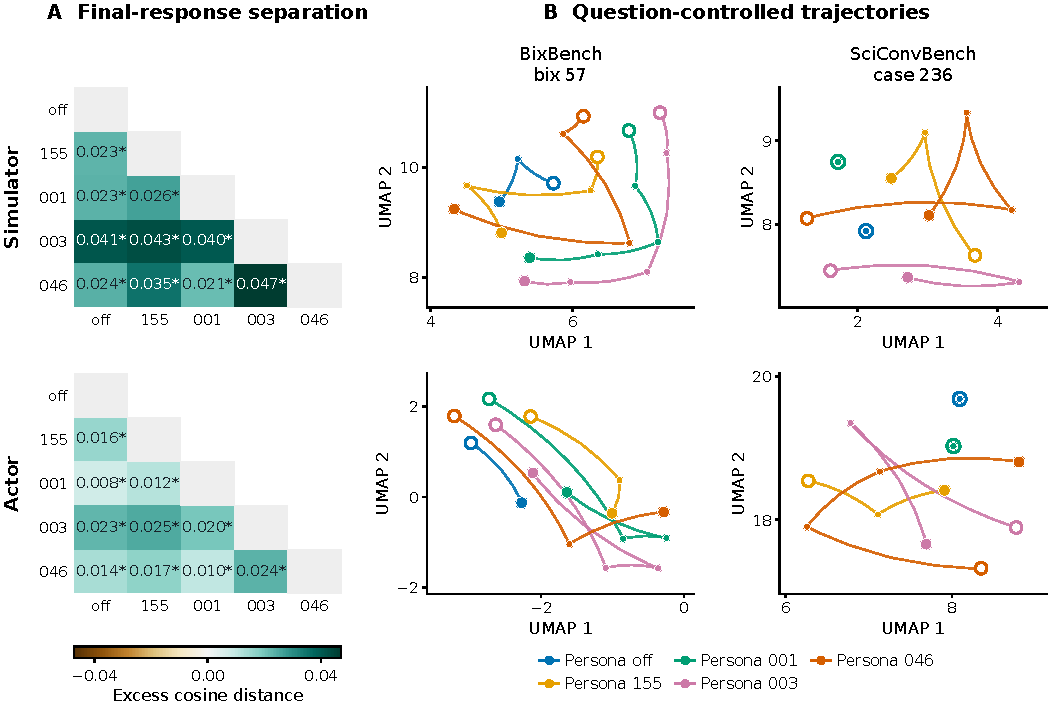
\includegraphics[width=0.75\linewidth]{figures/semantic.pdf}
% Source: Experiment/01_behavioral_diversity/SEMANTIC_FIGURE_CAPTION.md.
\caption{\textbf{Semantic separation and interaction trajectories.}
\textbf{A,} Final-response semantic separation for simulators (top)
and actors (bottom); stars indicate Holm-adjusted $p<0.05$.
\textbf{B,} Example UMAP trajectories for BixBench and SciConvBench.
Hollow circles mark starts, filled circles mark ends, and small dots
mark intermediate messages; overlapping start/end markers denote a single
message.}
\label{fig:semantic-diversity}
\end{figure}

Researcher personas were associated with distinct final responses from both
the simulator and the actor (\figref{fig:semantic-diversity}A).
We compared Qwen3-Embedding-0.6B~\cite{zhang2025qwen3embedding} embeddings within each
domain, measured separation relative to within-persona variation across
questions, and weighted the four domains equally. All
ten persona-pair comparisons showed positive separation in each role
(Holm-adjusted $p<0.05$ in question-wise persona-label permutation
tests~\cite{phipson2010permutation,holm1979sequential}). The effect of personas at the same time extended to the actor's final responses, even though the actor
encountered the researcher profile only through conversation.

Persona diversity appeared in both the intermediate messages and the
overall course of interaction (\figref{fig:semantic-diversity}B).
In BixBench, both simulator and actor trajectories followed distinct paths
with similar overall movement and partial convergence in the
UMAP~\cite{mcinnes2018umap} projection. The shared task thus elicited a
recognizable progression across personas, while the messages produced
along the way remained different. In SciConvBench, the simulator
trajectories differed in their overall patterns, and the corresponding
actor trajectories were distinct as well. These examples illustrate how
diverse researcher behavior was reflected in the agent's responses
throughout the interaction.

Persona-conditioned interactions also drew the actor into more proactive
participation in multi-turn scientific work. The BixBench example involved more interaction iterations
under every persona than under persona off. In SciConvBench, personas 155,
003, and 046 involved three or four interaction iterations, compared with
one iteration for persona off. During these conversations, the actor pursued
specific questions: under persona 046, it successively clarified
the starting structure, magnetic configuration, external pressure, and
convergence criteria. This progression from a brief interaction to targeted
follow-up questions makes the agent an active participant in specifying
how the task should proceed. Such participation is valuable in scientific
collaboration, where initial requests can leave consequential assumptions
and preferences implicit. Continued dialogue gives the researcher and
agent opportunities to make those choices explicit, resolve uncertainty,
and incorporate feedback before committing to an approach.

\subsection{Researcher Profiles Elicit Different Communication Patterns}
\label{sec:behavioral-results}

Profiles that favor detailed communication were accompanied by more
extensive output from both the simulator and the actor
(\figref{fig:pairwise-behavior}A,B). Relative to persona off, personas 155
and 003 elicited an additional 1.12 and 0.61 thousand actor tokens per
episode, respectively. Simulator output also increased under both
profiles; all four comparisons had Holm-adjusted $p<0.05$. These
comparisons matched questions and trials before averaging across
benchmarks. The contrast also appeared between personas: actor output
under 155 and 003 exceeded that under persona 001, whose profile favors
brief, direct communication. Researcher preferences were thus reflected
in how much the agent produced in response, extending the behavioral
variation beyond the simulator itself.

The clearest differences appeared in communication volume. Clarification
recall varied by $-0.28$ to $4.55$ percentage points across persona pairs,
and tool use by $-0.54$ to $0.28$ calls per episode
(\figref{fig:pairwise-behavior}C,D); neither metric showed a pairwise
difference at Holm-adjusted $p<0.05$. These patterns give the benchmark
contrasting communication demands: detailed, accuracy-oriented guidance
under persona 155, concrete explanations under persona 003, and concise
responses under persona 001. Evaluating these settings together makes
responsiveness to researcher preferences an observable part of scientific
collaboration.

% Source: Experiment/01_behavioral_diversity/behavioral_analysis.ipynb,
% figures/compact_behavior/pairwise_behavior_four.pdf; COMPACT_BEHAVIOR.md.
\begin{figure}[!htbp]
    \centering
    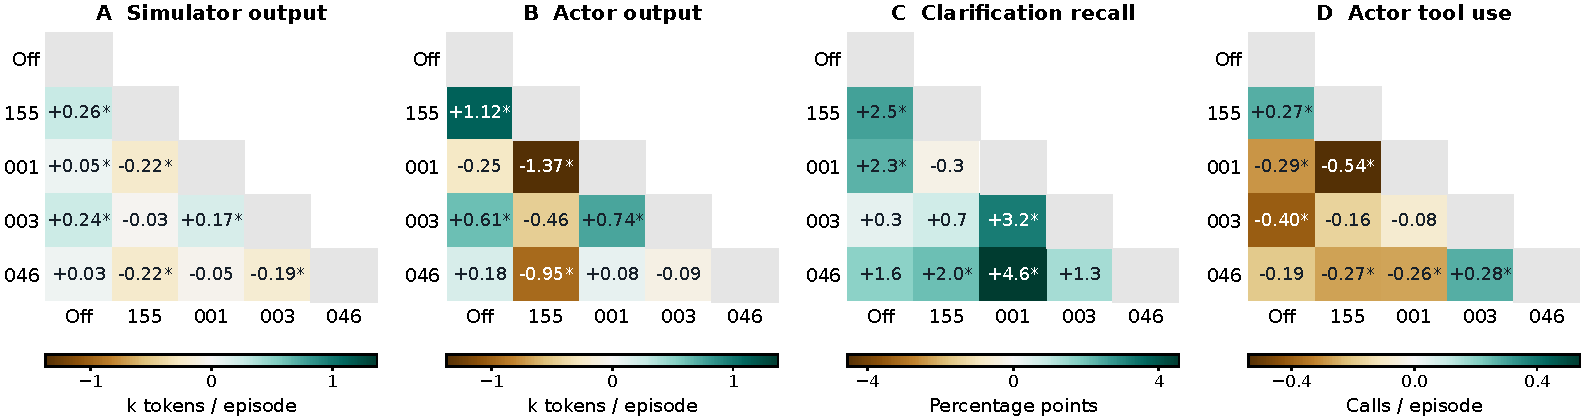
\includegraphics[width=\linewidth]{figures/pairwise_behavior_four.pdf}
    \caption{\textbf{Pairwise behavioral differences.}
Cells show row minus column. \textbf{A, B,} Simulator and actor output
(thousands of tokens per episode). \textbf{C,} SciConvBench clarification
recall (percentage points). \textbf{D,} Actor tool calls per episode.
Stars: \textbf{A, B,} Holm-adjusted $p<0.20$; \textbf{C, D,}
absolute differences above 2 percentage points and 0.2 calls, respectively.}
\label{fig:pairwise-behavior}
\end{figure}


\Needspace{18\baselineskip}
\subsection{Interaction Behavior beyond Final Scores}
\label{sec:interaction-outcomes}

\begin{wrapfigure}{R}{0.58\textwidth}
\vspace{-\intextsep}
\centering
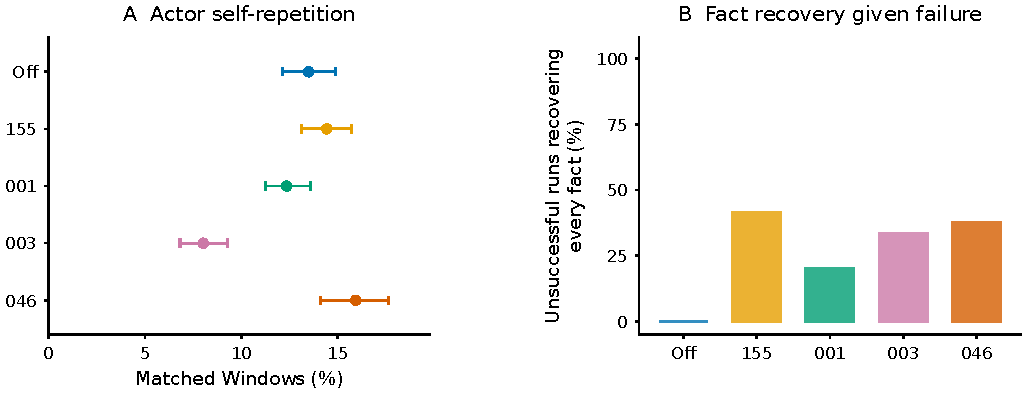
\includegraphics[width=\linewidth]{figures/metric_suite_AB.pdf}
\caption{\textbf{Interaction metrics across researcher personas.}
\textbf{A,} Actor self-repetition; bars show pointwise 95\% study-cluster
confidence intervals. \textbf{B,} Complete-fact recovery among failed
SciConvBench disambiguation episodes.}
\label{fig:metric-suite}
\end{wrapfigure}

The actor returned to its earlier wording to different degrees depending
on the researcher persona (\figref{fig:metric-suite}A). Self-repetition
was 8.03\% under persona 003, compared with 13.50\% for persona off
and 15.94\% under persona 046. These differences are relevant to
conversational mode collapse, where interactions become concentrated in
a few recurring response patterns. CORE evaluates this phenomenon
jointly through mode diversity, lexical repetition, and semantic
stagnation~\cite{pandey2026core}. Extended closed-loop LLM studies
also report semantic collapse, with meanings converging even as surface
wording varies~\cite{kong2026semanticcollapse}. This motivates assessing
self-repetition alongside semantic diversity
(\secref{sec:semantic-results}). In scientific collaboration, avoiding
unnecessary repetition preserves space for targeted clarification,
updated interpretations, and revision of the scientific approach.
The lower self-repetition under persona 003 highlights a setting in
which less of the actor's output reuses its earlier language.
The observed interaction lengths further motivate evaluating multi-turn
scientific work (\figref{fig:interaction-performance}). Every setting received score
contributions from episodes completing after the second iteration. For
persona 003, the cumulative contribution rose from 37.49 at iteration two
to 48.69 at iteration six as later-completing episodes were included.

Information recovery revealed progress during multi-turn scientific work,
including in episodes that ultimately failed (\figref{fig:metric-suite}B).
Within each setting's failed SciConvBench disambiguation episodes,
the case-averaged rate of recovering all required facts ranged from
20.0\% to 41.7\% across the four personas, compared with 0\% for
persona off. The persona-conditioned episodes with complete recovery
contained four to ten interaction iterations, during which the actor
elicited every annotated missing fact before termination. This identifies
a concrete intermediate accomplishment within unsuccessful tasks:
establishing the full factual context needed to formulate a scientific
response. Final scores alone would leave this information-gathering
progress unreported.

\section{Discussion and Conversation Case Studies}
\label{sec:discussion}

\sectiontodo{Draft the discussion and conversation case studies.}

\FloatBarrier
\Needspace{11\baselineskip}
\section{Conclusion}
\label{sec:conclusion}

\sectiontodo{Draft the conclusion.}

\section{Limitations and Responsible Use}
\label{sec:limitations}

\todo{Discuss simulated rather than human collaborators; a small, outcome-selected persona panel; full-profile confounding; language and domain differences; inconsistent profile attributes; source-study dependence; benchmark/field confounding; three repeats; model-based grading uncertainty; and technical missingness.}

\todo{Describe profile/data provenance and licensing, protection of credentials and private evaluator references, and limits on interpreting demographic attributes. Do not claim that these profiles represent real people or demographic groups.}


% Add verified bibliography entries and citations during drafting.
\bibliographystyle{plainnat}
\bibliography{references}

\clearpage
\appendix
\section{Supplementary Material}
\label{app:supplementary}

\sectiontodo{Add supplementary material.}


\end{document}
